\documentclass[11pt,preprint, authoryear]{elsarticle}

\usepackage{lmodern}
%%%% My spacing
\usepackage{setspace}
\setstretch{1.2}
\DeclareMathSizes{12}{14}{10}{10}

% Wrap around which gives all figures included the [H] command, or places it "here". This can be tedious to code in Rmarkdown.
\usepackage{float}
\let\origfigure\figure
\let\endorigfigure\endfigure
\renewenvironment{figure}[1][2] {
    \expandafter\origfigure\expandafter[H]
} {
    \endorigfigure
}

\let\origtable\table
\let\endorigtable\endtable
\renewenvironment{table}[1][2] {
    \expandafter\origtable\expandafter[H]
} {
    \endorigtable
}


\usepackage{ifxetex,ifluatex}
\usepackage{fixltx2e} % provides \textsubscript
\ifnum 0\ifxetex 1\fi\ifluatex 1\fi=0 % if pdftex
  \usepackage[T1]{fontenc}
  \usepackage[utf8]{inputenc}
\else % if luatex or xelatex
  \ifxetex
    \usepackage{mathspec}
    \usepackage{xltxtra,xunicode}
  \else
    \usepackage{fontspec}
  \fi
  \defaultfontfeatures{Mapping=tex-text,Scale=MatchLowercase}
  \newcommand{\euro}{€}
\fi

\usepackage{amssymb, amsmath, amsthm, amsfonts}

\def\bibsection{\section*{References}} %%% Make "References" appear before bibliography


\usepackage[round]{natbib}

\usepackage{longtable}
\usepackage[margin=2.3cm,bottom=2cm,top=2.5cm, includefoot]{geometry}
\usepackage{fancyhdr}
\usepackage[bottom, hang, flushmargin]{footmisc}
\usepackage{graphicx}
\numberwithin{equation}{section}
\numberwithin{figure}{section}
\numberwithin{table}{section}
\setlength{\parindent}{0cm}
\setlength{\parskip}{1.3ex plus 0.5ex minus 0.3ex}
\usepackage{textcomp}
\renewcommand{\headrulewidth}{0.2pt}
\renewcommand{\footrulewidth}{0.3pt}

\usepackage{array}
\newcolumntype{x}[1]{>{\centering\arraybackslash\hspace{0pt}}p{#1}}

%%%%  Remove the "preprint submitted to" part. Don't worry about this either, it just looks better without it:
\makeatletter
\def\ps@pprintTitle{%
  \let\@oddhead\@empty
  \let\@evenhead\@empty
  \let\@oddfoot\@empty
  \let\@evenfoot\@oddfoot
}
\makeatother

 \def\tightlist{} % This allows for subbullets!

\usepackage{hyperref}
\hypersetup{breaklinks=true,
            bookmarks=true,
            colorlinks=true,
            citecolor=blue,
            urlcolor=blue,
            linkcolor=blue,
            pdfborder={0 0 0}}


% The following packages allow huxtable to work:
\usepackage{siunitx}
\usepackage{multirow}
\usepackage{hhline}
\usepackage{calc}
\usepackage{tabularx}
\usepackage{booktabs}
\usepackage{caption}


\newenvironment{columns}[1][]{}{}

\newenvironment{column}[1]{\begin{minipage}{#1}\ignorespaces}{%
\end{minipage}
\ifhmode\unskip\fi
\aftergroup\useignorespacesandallpars}

\def\useignorespacesandallpars#1\ignorespaces\fi{%
#1\fi\ignorespacesandallpars}

\makeatletter
\def\ignorespacesandallpars{%
  \@ifnextchar\par
    {\expandafter\ignorespacesandallpars\@gobble}%
    {}%
}
\makeatother

\newlength{\cslhangindent}
\setlength{\cslhangindent}{1.5em}
\newenvironment{CSLReferences}%
  {\setlength{\parindent}{0pt}%
  \everypar{\setlength{\hangindent}{\cslhangindent}}\ignorespaces}%
  {\par}


\urlstyle{same}  % don't use monospace font for urls
\setlength{\parindent}{0pt}
\setlength{\parskip}{6pt plus 2pt minus 1pt}
\setlength{\emergencystretch}{3em}  % prevent overfull lines
\setcounter{secnumdepth}{5}

%%% Use protect on footnotes to avoid problems with footnotes in titles
\let\rmarkdownfootnote\footnote%
\def\footnote{\protect\rmarkdownfootnote}
\IfFileExists{upquote.sty}{\usepackage{upquote}}{}

%%% Include extra packages specified by user
\usepackage{booktabs}
\usepackage{longtable}
\usepackage{array}
\usepackage{multirow}
\usepackage{wrapfig}
\usepackage{float}
\usepackage{colortbl}
\usepackage{pdflscape}
\usepackage{tabu}
\usepackage{threeparttable}
\usepackage{threeparttablex}
\usepackage[normalem]{ulem}
\usepackage{makecell}
\usepackage{xcolor}

%%% Hard setting column skips for reports - this ensures greater consistency and control over the length settings in the document.
%% page layout
%% paragraphs
\setlength{\baselineskip}{12pt plus 0pt minus 0pt}
\setlength{\parskip}{12pt plus 0pt minus 0pt}
\setlength{\parindent}{0pt plus 0pt minus 0pt}
%% floats
\setlength{\floatsep}{12pt plus 0 pt minus 0pt}
\setlength{\textfloatsep}{20pt plus 0pt minus 0pt}
\setlength{\intextsep}{14pt plus 0pt minus 0pt}
\setlength{\dbltextfloatsep}{20pt plus 0pt minus 0pt}
\setlength{\dblfloatsep}{14pt plus 0pt minus 0pt}
%% maths
\setlength{\abovedisplayskip}{12pt plus 0pt minus 0pt}
\setlength{\belowdisplayskip}{12pt plus 0pt minus 0pt}
%% lists
\setlength{\topsep}{10pt plus 0pt minus 0pt}
\setlength{\partopsep}{3pt plus 0pt minus 0pt}
\setlength{\itemsep}{5pt plus 0pt minus 0pt}
\setlength{\labelsep}{8mm plus 0mm minus 0mm}
\setlength{\parsep}{\the\parskip}
\setlength{\listparindent}{\the\parindent}
%% verbatim
\setlength{\fboxsep}{5pt plus 0pt minus 0pt}



\begin{document}



\begin{frontmatter}  %

\title{Question 5: Google}

% Set to FALSE if wanting to remove title (for submission)




\author[Add1]{Andrew Hyde\footnote{\textbf{Contributions:}
  \newline \emph{The author would like to thank Stack Overflow.}}}
\ead{23365935@sun.ac.za}





\address[Add1]{Stellenbosch University, South Africa}

\cortext[cor]{Corresponding author: Andrew Hyde\footnote{\textbf{Contributions:}
  \newline \emph{The author would like to thank Stack Overflow.}}}

\begin{abstract}
\small{
Background information into App design trends.
}
\end{abstract}

\vspace{1cm}





\vspace{0.5cm}

\end{frontmatter}



%________________________
% Header and Footers
%%%%%%%%%%%%%%%%%%%%%%%%%%%%%%%%%
\pagestyle{fancy}
\chead{}
\rhead{}
\lfoot{}
\rfoot{\footnotesize Page \thepage}
\lhead{}
%\rfoot{\footnotesize Page \thepage } % "e.g. Page 2"
\cfoot{}

%\setlength\headheight{30pt}
%%%%%%%%%%%%%%%%%%%%%%%%%%%%%%%%%
%________________________

\headsep 35pt % So that header does not go over title




\hypertarget{application-categories-that-generate-the-most-revemue.}{%
\section{Application Categories that Generate the most
Revemue.}\label{application-categories-that-generate-the-most-revemue.}}

From the graph below, one can see that the three categories of
applications with the largest revenues on the Google Store are
Lifestyle, Finance and Photography. This is likely due to the fact that
these applications would appeal to the most users. I would issue
caution, when considering developing a new app in any of these three
categories as there is a large amount of competition and a new app may
struggle to gain traction with incumbent apps having the first mover
advantage.

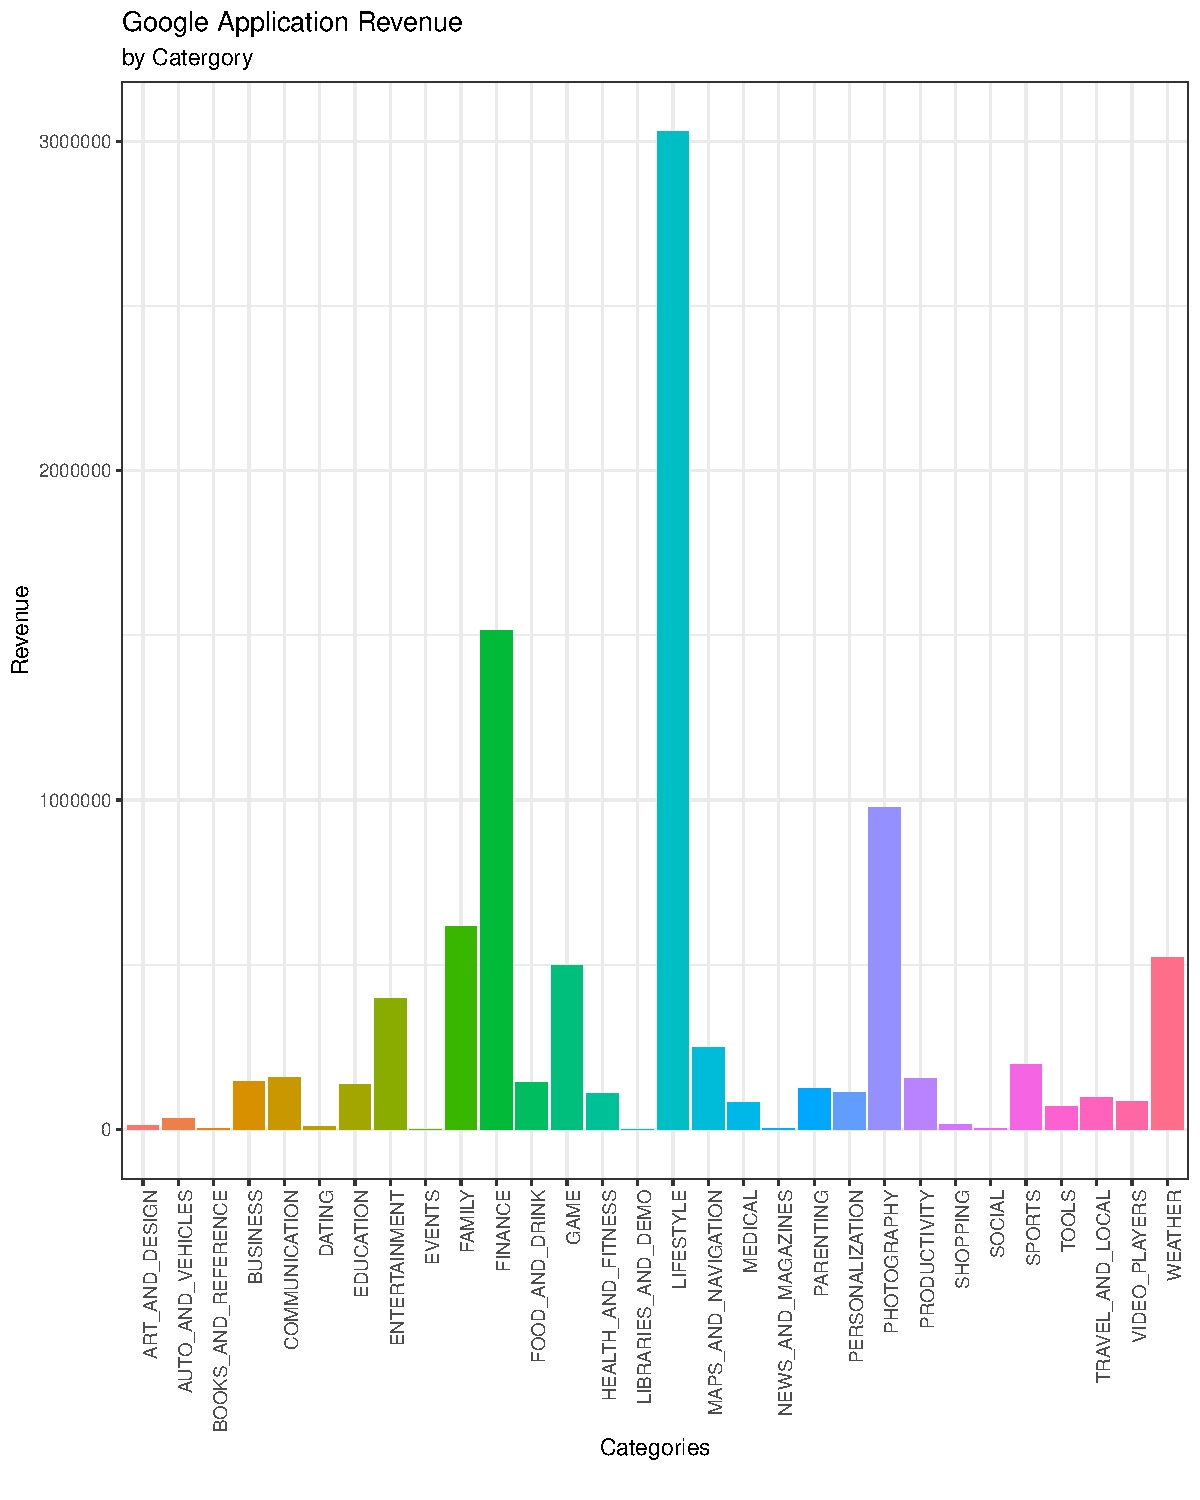
\includegraphics{Question5_files/figure-latex/unnamed-chunk-1-1.pdf}

\newpage

The table below, displays the mean statistics of price, number of
installs, revenue, size per category. In terms of average price, the
three most expensive categories are Finance, Lifestyle and Events.

\begin{table}

\caption{\label{tab:unnamed-chunk-2}Summary of Application Statistics per Catergory}
\centering
\begin{tabular}[t]{c|c|c|c|c}
\hline
Category & Price \$ & Installs & Revenue & Size\\
\hline
\cellcolor{gray!6}{ART\_AND\_DESIGN} & \cellcolor{gray!6}{1.990000} & \cellcolor{gray!6}{5333.3333} & \cellcolor{gray!6}{10613.333} & \cellcolor{gray!6}{5.200000}\\
\hline
AUTO\_AND\_VEHICLES & 4.490000 & 16716.6667 & 33382.833 & NA\\
\hline
\cellcolor{gray!6}{BOOKS\_AND\_REFERENCE} & \cellcolor{gray!6}{4.277500} & \cellcolor{gray!6}{832.7143} & \cellcolor{gray!6}{3222.384} & \cellcolor{gray!6}{NA}\\
\hline
BUSINESS & 13.233571 & 29483.9286 & 146324.518 & NA\\
\hline
\cellcolor{gray!6}{COMMUNICATION} & \cellcolor{gray!6}{3.079259} & \cellcolor{gray!6}{50372.2222} & \cellcolor{gray!6}{157309.796} & \cellcolor{gray!6}{NA}\\
\hline
DATING & 4.090000 & 2070.0000 & 8294.300 & NA\\
\hline
\cellcolor{gray!6}{EDUCATION} & \cellcolor{gray!6}{4.656667} & \cellcolor{gray!6}{34000.0000} & \cellcolor{gray!6}{136326.667} & \cellcolor{gray!6}{43.666667}\\
\hline
ENTERTAINMENT & 3.990000 & 100000.0000 & 399000.000 & NA\\
\hline
\cellcolor{gray!6}{EVENTS} & \cellcolor{gray!6}{109.990000} & \cellcolor{gray!6}{1.0000} & \cellcolor{gray!6}{109.990} & \cellcolor{gray!6}{6.700000}\\
\hline
FAMILY & 12.871330 & 112616.0319 & 615710.773 & NA\\
\hline
\cellcolor{gray!6}{FINANCE} & \cellcolor{gray!6}{170.637059} & \cellcolor{gray!6}{10917.7647} & \cellcolor{gray!6}{1513334.058} & \cellcolor{gray!6}{NA}\\
\hline
FOOD\_AND\_DRINK & 4.240000 & 30000.0000 & 142200.000 & NA\\
\hline
\cellcolor{gray!6}{GAME} & \cellcolor{gray!6}{3.467195} & \cellcolor{gray!6}{256097.1341} & \cellcolor{gray!6}{496202.888} & \cellcolor{gray!6}{NA}\\
\hline
HEALTH\_AND\_FITNESS & 4.208750 & 35881.8750 & 107816.806 & NA\\
\hline
\cellcolor{gray!6}{LIBRARIES\_AND\_DEMO} & \cellcolor{gray!6}{0.990000} & \cellcolor{gray!6}{100.0000} & \cellcolor{gray!6}{99.000} & \cellcolor{gray!6}{4.700000}\\
\hline
LIFESTYLE & 124.256316 & 62058.4211 & 3030733.653 & NA\\
\hline
\cellcolor{gray!6}{MAPS\_AND\_NAVIGATION} & \cellcolor{gray!6}{5.390000} & \cellcolor{gray!6}{24220.0000} & \cellcolor{gray!6}{248157.800} & \cellcolor{gray!6}{NA}\\
\hline
MEDICAL & 12.990476 & 7807.9333 & 81659.483 & NA\\
\hline
\cellcolor{gray!6}{NEWS\_AND\_MAGAZINES} & \cellcolor{gray!6}{1.990000} & \cellcolor{gray!6}{2750.0000} & \cellcolor{gray!6}{3222.500} & \cellcolor{gray!6}{14.900000}\\
\hline
PARENTING & 4.790000 & 25050.0000 & 124979.500 & NA\\
\hline
\cellcolor{gray!6}{PERSONALIZATION} & \cellcolor{gray!6}{1.865488} & \cellcolor{gray!6}{51936.5122} & \cellcolor{gray!6}{113255.458} & \cellcolor{gray!6}{NA}\\
\hline
PHOTOGRAPHY & 6.202857 & 184701.9048 & 977512.748 & NA\\
\hline
\cellcolor{gray!6}{PRODUCTIVITY} & \cellcolor{gray!6}{8.961786} & \cellcolor{gray!6}{50430.5357} & \cellcolor{gray!6}{154049.105} & \cellcolor{gray!6}{NA}\\
\hline
SHOPPING & 2.740000 & 5050.0000 & 15074.500 & 3.400000\\
\hline
\cellcolor{gray!6}{SOCIAL} & \cellcolor{gray!6}{5.323333} & \cellcolor{gray!6}{2000.0000} & \cellcolor{gray!6}{1980.000} & \cellcolor{gray!6}{6.533333}\\
\hline
SPORTS & 4.166667 & 51825.6250 & 196092.165 & NA\\
\hline
\cellcolor{gray!6}{TOOLS} & \cellcolor{gray!6}{3.426282} & \cellcolor{gray!6}{22146.6795} & \cellcolor{gray!6}{70061.802} & \cellcolor{gray!6}{NA}\\
\hline
TRAVEL\_AND\_LOCAL & 4.162500 & 15255.0000 & 95958.700 & NA\\
\hline
\cellcolor{gray!6}{VIDEO\_PLAYERS} & \cellcolor{gray!6}{2.615000} & \cellcolor{gray!6}{17750.0000} & \cellcolor{gray!6}{83822.500} & \cellcolor{gray!6}{NA}\\
\hline
WEATHER & 4.052500 & 101500.0000 & 522672.500 & NA\\
\hline
\end{tabular}
\end{table}

\bibliography{Tex/ref}





\end{document}
